\chapter{Zvolené řešení a jeho vyhodnocení}\label{chapter:choosen_solution}
Finálním vybraným řešením pro vyhodnocení je řešení s~termokamerou a algoritmem dynamického odčítání pozadí. Detaily algoritmu jsou uvedeny v~\ref{section:background_substract_solution} a zde je uvedeno pouze jeho stručné shrnutí. 

\section{Shrnutí řešení}
V~paměti je průběžně aktualizováno pozadí vůči kterému se vyhodnocuje právě načtený snímek. V~případě, že je snímek detekován jako pozadí, aktualizuje se s~jeho pomocí to v~paměti. V~opačném případě je získané popředí snímku, na kterém se dále segmentuje ruka. Pomocí invertované masky ruky je získáno popředí bez ruky, na kterém proběhne redukce artefaktů ve formě šumu a jako poslední krok je výpočet atributů pro klasifikaci.

\section{Volba atributů}\label{section:attributes}
Pro řešení bylo zvoleno celkem 20 atributů zaměřující se na vlastnosti kontur. Atributy související s~jasem, histogramem a podobnými vlastnostmi obrazu nebyly použity, protože výstup z~kamery se v~čase mění a není možné zajistit jeho stabilitu.

Zvolené atributy jsou rozděleny do dvou skupin. Na atributy týkající se vlastností největší nalezené kontury a souhrnné atributy všech nalezených kontur. Atributy vypočítávány na největší nalezené kontuře jsou:
\begin{description}
\item [Délka kontury (Perimeter)]
\item [Plocha kontury (Area)]
\item [Minimální průměr vepsané kružnice (Minimum diameter)]
\item [Maximální průměr vepsané kružnice (Maximum diameter)]
\item [Délka konvexní obálky (Convex perimeter)]
\item [Plocha konvexní obálky (Convex area)]
\item [Formfaktor (Formfactor)] získán jako 
    \begin{equation}
        \frac{4 \times \pi \times Area}{Perimeter^{2}}        
    \end{equation}
\item [Kulatost (Roundness)] získána jako 
    \begin{equation}
        \frac{4 \times Area}{\pi \times \text{Maximum diameter}^{2}}
    \end{equation}
\item [Poměr stran (Aspect ratio)] získán jako
	\begin{equation}
        \frac{\text{Maximum diameter}}{\text{Minimum diameter}}
	\end{equation}
\item [Konvexita (Convexity)] získána jako
	\begin{equation}
        \frac{\text{Convex perimeter}}{Perimeter}
	\end{equation}
\item [Pevnost (Solidity)] získána jako
	\begin{equation}
        \frac{Area}{\text{Convex area}}
	\end{equation}
\item [Kompaktnost (Compactness)] získána jako
	\begin{equation}
        \frac{\sqrt{\frac{4}{\pi} \times Area}}{\text{Maximum diameter}}
	\end{equation}
\item [Rozsah (Extent)] získán jako
	\begin{equation}
        \frac{Area}{\text{Maximum diameter} \times \text{Minimum diameter}} .
	\end{equation}
\end{description}
Atributy vypočítávané na všech nalezených konturách jsou:

\begin{description}
\item [Počet kontur]
\item [Součet ploch kontur]
\item [Minimální plocha kontury]
\item [Průměrná plocha kontury]
\item [Součet délek kontur]
\item [Minimální délka kontury]
\item [Průměrná délka kontury.]
\end{description}


\section{Rozdělení snímků do tříd}
Před klasifikaci, je nejdříve nutné snímky rozdělit do několika skupin. Klasifikačními skupinami jsou prázdná ruka a ruka se zbožím, ale pro správnou funkčnost uvedeného algoritmu je ještě nutné v~paměti uchovávat pozadí. Čím více snímků pozadí bude při vyhodnocování k~dispozici, tím budou výsledky přesnější.

Snímky jsou uchovávány jako binární soubory obsahující data v~podobě signálů, takže je nutno vytvořit speciální aplikaci pro jejich zobrazení a následné rozřazení do tříd. Pomocí této aplikace bylo ručně anotováno celkem 910 snímků prázdné ruky a 973 snímků ruky se zbožím. Všechna anotovaná pozadí byla získána pomocí aplikace s~algoritmy a ručně zkontrolovány pomocí aplikace pro anotování. Těchto pozadí je celkem 2173.

Navzdory tomu, že byly při práci využity dvě kamery, budou klasifikovány snímky pouze z~kamery (13 mm). Je to z~toho důvodu, že v~nasnímaných datasetech kamery (25 mm) se vyskytuje množství chyb, které vznikaly nevypočitatelně, kvůli její technické závadě. 

Celkem se tedy bude vyhodnocovat 1244 anotovaných snímků z~kamery (13 mm), z~toho 741 snímků ruky a 503 snímků ruky se zbožím, s~pomocí 2031 snímků pozadí.


\section{Klasifikace}
Před samotnou klasifikací jsou ještě jednotlivé hodnoty atributů normalizovány. Následně je spouštěna detekce anomálií a z~datasetu jsou některé záznamy odstraněny. Odstraněni probíhá pokud se součet délek kontur přibližuje celkové možné ploše obrazového pole. Tyto záznamy jsou očividně chybné a vznikají nejčastěji ihned po NUC, kdy ještě není dostatečně aklimatizováno uložené pozadí a při operaci odčítání pozadí se celý snímek bere jako popředí (ilustrováno v~předchozí kapitole \ref{section:background_substract_problems}). Tyto případy jsou považovány za chyby měření a jsou odstraněny.

Ke klasifikaci je využit program RapidMiner, který poskytuje velké množství různých klasifikátorů a ostatních užitečných nástrojů pro data mining. 

\section{Výsledky}
K~vyhodnocení výsledků je použita 10-násobná křížová validace (10-fold cross validation) a bylo vyzkoušeno celkem 10 různých klasifikátorů. Výsledky jednotlivých klasifikátorů jsou uvedeny v~tabulce \ref{table:classificators_result}. Jako nejpřesnější klasifikátor se jeví neuronová síť s~celkovou přesností 88.66\%. Podrobnější výsledky k~tomuto klasifikátoru je možné vidět v~matici záměn \ref{table:neural_net_result}.

\begin{table}[h]
  \centering
  \begin{tabular}{|c|c|c|c|}
  \hline
  \rowcolor{Blue}
  \color{White}\textbf{Klasifikátor} & \color{White}\textbf{Prázdná ruka} & \color{White}\textbf{Ruka se zbožím} & \color{White}\textbf{Celková přesnost} \\ \hline
  Naivní bayes & 91.29\% & 78.31\% & 85.37\% \\ \hline
  3-NN & 88.19\% & 88.39\% & 88.27\% \\ \hline
  5-NN & 87.33\% & 88.57\% & 87.78\%\\ \hline
  10-NN & 87.40\% & 89.52\% & 88.18\% \\ \hline
  Lineární regrese & 91.29\% & 78.31\% & 85.37\% \\ \hline
  SVM & 89.36\% & 85.98\% & 88.02\% \\ \hline
  Rozhodovací strom & 87.12\% & 87.39\% & 87.22\%  \\ \hline
  Rozhodovací les & 89.31\% & 86.83\% & 88.35\% \\ \hline
  GBT & 86.83\% & 89.04\% & 87.62\%  \\ \hline
  Neuronová síť & 87.91\% & 90.39\% & 88.83\% \\ \hline
  \end{tabular}
  \caption{Tabulka pozitivní prediktivní hodnoty jednotlivých tříd (class precision) a celkové přesnosti (accuracy) jednotlivých klasifikátorů}
  \label{table:classificators_result}
\end{table}


\begin{table}[]
  \catcode`\-=12
  \centering
  \begin{tabular}{cl|l|l|l}
    \cline{3-4}
    \multicolumn{1}{l}{} & \multicolumn{1}{c|}{} & \multicolumn{2}{c|}{\cellcolor{Blue}\color{White}\textbf{Skutečnost}} &  \\ \cline{3-5} 
     & \multicolumn{1}{c|}{} & prázdná ruka & ruka se zbožím & \multicolumn{1}{l|}{\textit{class precision}} \\ \hline
    \multicolumn{1}{|c|}{\cellcolor{Blue}} & prázdná ruka & 691 & 95 & \multicolumn{1}{l|}{87.91\%} \\ \cline{2-5} 
    \multicolumn{1}{|c|}{\multirow{-2}{*}{\cellcolor{Blue}\color{White}\textbf{Klasifikace}}} & ruka se zbožím & 44 & 414 & \multicolumn{1}{l|}{90.39\%} \\ \hline
    \multicolumn{1}{l|}{\textit{}} & \textit{class recall} & 94.01\% & 81.34\% &  \\ \cline{2-4}
  \end{tabular}
  \caption{Matice záměn neuronové sítě vyhodnocena pomocí 10-násobné křížové validace}
  \label{table:neural_net_result}
\end{table}

\section{Příklady klasifikovaných snímků}
V~této části je uvedeno několik názorných příkladů klasifikace, tak jak je určila neuronová síť. Pro větší názornost jsou tyto snímky již předzpracovány. Na jednotlivých snímcích si lze též všimnout, jak se snímané prostředí poměrně zásadně mění. Jsou uvedeny příklady správně klasifikovaných ( \ref{fig:empty_hand_correct}, \ref{fig:hand_with_goods_correct}), ale i chybně klasifikovaných (\ref{fig:empty_hand_wrong}, \ref{fig:hand_with_goods_wrong}). 

\begin{figure}[h]
  \centering
  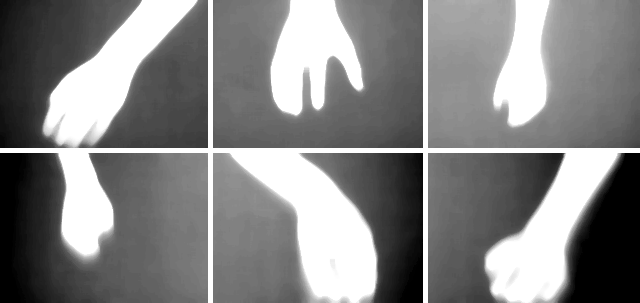
\includegraphics[width=0.8\textwidth]{images/empty_hand_correct.png}
  \caption{Příklady správně klasifikovaných snímků kategorie prázdná ruka}
  \label{fig:empty_hand_correct}
\end{figure} 

\begin{figure}[h]
  \centering
  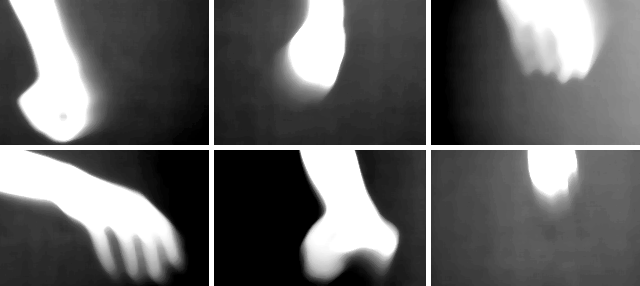
\includegraphics[width=0.8\textwidth]{images/empty_hand_wrong.png}
  \caption{Příklady klasifikovaných snímků jako ruka se zbožím, ale ve skutečnosti prázdná ruka}
  \label{fig:empty_hand_wrong}
\end{figure} 

\begin{figure}[h]
  \centering
  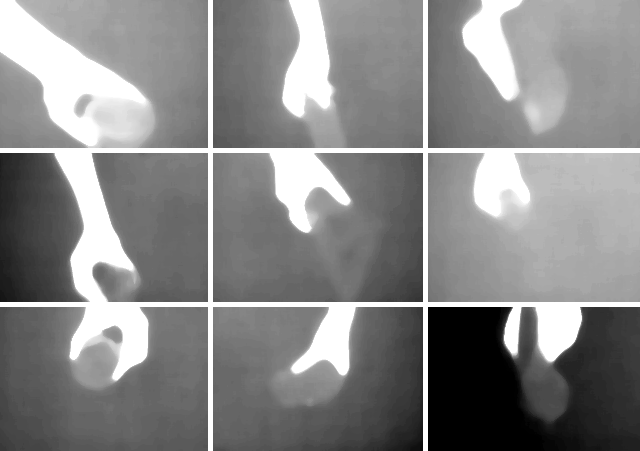
\includegraphics[width=0.8\textwidth]{images/hand_with_goods_correct.png}
  \caption{Příklady správně klasifikovaných snímků kategorie ruka se zbožím}
  \label{fig:hand_with_goods_correct}
\end{figure} 

\begin{figure}[h]
  \centering
  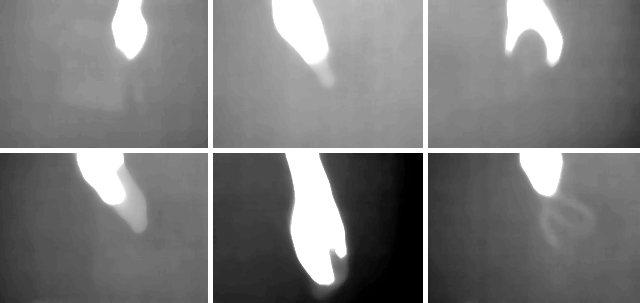
\includegraphics[width=0.8\textwidth]{images/hand_with_goods_wrong.png}
  \caption{Příklady klasifikovaných snímků jako prázdná ruka, ale ve skutečnosti ruka se zbožím}
  \label{fig:hand_with_goods_wrong}
\end{figure} 

	\subsection{Komentář ke klasifikaci snímků}
    Obecně by mělo být snadné detekovat ruku, protože na její teplotu se dá vždy spolehnout. Problém nastává při jejím rychlém pohybu, kdy pohybová neostrost zabrání jejímu správnému segmentování. Většina chybně klasifikovaných rukou jsou pohybově neostré snímky, případně snímky před kterými došlo ke změně pozadí, kdy se uložené pozadí ještě nestihlo adaptovat této změně.
    
    Z~chybně klasifikovaných snímků ruky se zbožím je zřejmé, že některé zboží mělo teplotu podobnou podlaze a na snímku je velmi obtížně rozlišitelné. Druhým případem je zboží, které je sice viditelné, ale má menší rozměry, takže po aplikaci morfologických operací již není rozpoznatelné.

